\documentclass[a4paper, 12pt]{article}
\usepackage[utf8]{inputenc}
\usepackage[francais]{babel}
\usepackage[pdftex]{graphicx}
\usepackage{hyperref}
\usepackage{titlesec}

\titleformat*{\section}{\LARGE\bfseries}
\titleformat*{\subsection}{\large\bfseries}

\begin{document}
\begin{titlepage}
\begin{center}

{\Large Université de Mons}\\[1ex]
{\Large Faculté des sciences}\\[1ex]
{\Large Département d'Informatique}\\[2.5cm]

\newcommand{\HRule}{\rule{\linewidth}{0.3mm}}
% Title
\HRule \\[0.3cm]
{ \LARGE \bfseries Quoridor \\[0.3cm]}
{ \LARGE \bfseries Rapport de projet \\[0.1cm]} % Commenter si pas besoin
\HRule \\[1.5cm]

% Author and supervisor
\begin{minipage}[t]{0.45\textwidth}
\begin{flushleft} \large
\emph{Professeur:}\\
Hadrien \textsc{Mélot}\\
\end{flushleft}
\end{minipage}
\begin{minipage}[t]{0.45\textwidth}
\begin{flushright} \large
\emph{Auteurs:} \\
Virgil \textsc{Surin} \\
Simon \textsc{Michel}
\end{flushright}
\end{minipage}\\[2ex]

\vfill

% Bottom of the page
\begin{center}
\begin{tabular}[t]{c c c}

\includegraphics[height=1.5cm]{logoumons.jpg} &
\hspace{0.3cm} &

\includegraphics[height=1.5cm]{logofs.jpg}
\end{tabular}
\end{center}~\\
 
{\large Année académique 2019-2020}

\end{center}
\end{titlepage}

\tableofcontents

\newpage

\section{Introduction}

Ce projet à pour objectif de ré-implémenter en Java le jeu de plateau Quoridor mais également de nous permettre d'apprendre à développer de A à Z une application fonctionnelle relativement importante en terme de taille et de complexité (pour notre niveau de première année du moins). \\
Ce projet est également l'occasion pour nous d'apprendre à nous organiser, à travailler en groupe mais également d'apprendre à chercher par nous même des solutions à des problèmes. \\
Afin de le mener à bien il nous a fallu du temps, beaucoup de réflexion mais aussi beaucoup de tests et d'essais. Nous avons crée plusieurs prototypes afin d'expérimenter des concepts, peser les pours et les contres pour au final arriver au résultat que vous avez sous vos yeux.

\section{Mode d'emploi}

Le jeu mode graphique du jeu se lance avec la commande \textit{gradle run} précédée d'un
\textit{gradle build}. Le menu se lance alors, vous pouvez choisir les paramètres de la
partie ou en charger une si une partie a déjà été sauvegardée. \\
Afin de déplacer votre pion, vous devez faire un clique gauche sur celui-ci, les différents déplacements possibles seront mis en évidence. En deuxième clique gauche sur la case souhaitée vous y déplacera. \\
Afin de placer des murs, maintenez le clique droit de la souris pour faire apparaître un mur fantôme. Placez le mur fantôme à l'endroit désiré et faites un clique gauche pour le placer. Un clique gauche ailleurs le fera disparaitre. \\
Vous pouvez à tout moment appuyer sur la touche \textit{ECHAP} du clavier pour faire apparaître le menu pause qui vous permet de sauvegarder ou de retourner au menu principal.

\section{Choix personnel}
\subsection{Le plateau et les murs}
Le premier choix que nous avons fait est certainement la façon dont nous allions gérer le plateau et les éléments qui allaient le composer et surtout comment s'occuper correctement
des murs. \\
Tout d'abord, nous avons fixé un système de coordonnée (y,x) où la case la plus en haut à gauche sera l'origine (0,0) et celle en bas à droite aura la coordonnée (t-1,t-1) où \textit{t} représente la taille du plateau (qui sera toujours carré). \\
Pour le murs, nous avons réfléchis et deux approches se sont présentées : 
\begin{itemize}
\item[•] Créer une grille avec des cases pions et des cases murs
\item[•] Ne faire qu'une grille pour pions et donner aux cases la possibilité de savoir sur quel côté il y un mur.
\end{itemize}
Nous avons choisi après longue réflexion la deuxième solution. Elle nous semblaient plus simple car elle ne nécessitait pas de créer plusieurs types de cases différentes. De plus, cette solution demande uniquement une grille simple qui représente le plateau et il nous semblait aussi plus simple d'interroger la case pour savoir si elle possède un mur dans une direction donnée que de chercher dans une grille parallèle. Également, le déplacement nous semblait plus naturel à implémenter : \\
\textit{e.g :} pour faire un déplacement vers la droite il suffit d'ajouter 1 en abscisse. \\
Pour placer les murs sur le plateau, étant donné que nous n'avions pas de grille spéciale pour ça, nous avons adopté la convention suivante : \\
\begin{itemize}
\item[•] un mur se pose uniquement sur le côté droit ou le côté supérieur d'une case.
\item[•] un mur posé sur le côté droit sera vertical et ira vers le haut.
\item[•] un mur posé sur le côté supérieur sera horizontal et ira vers la droite.
\end{itemize}
\begin{center}
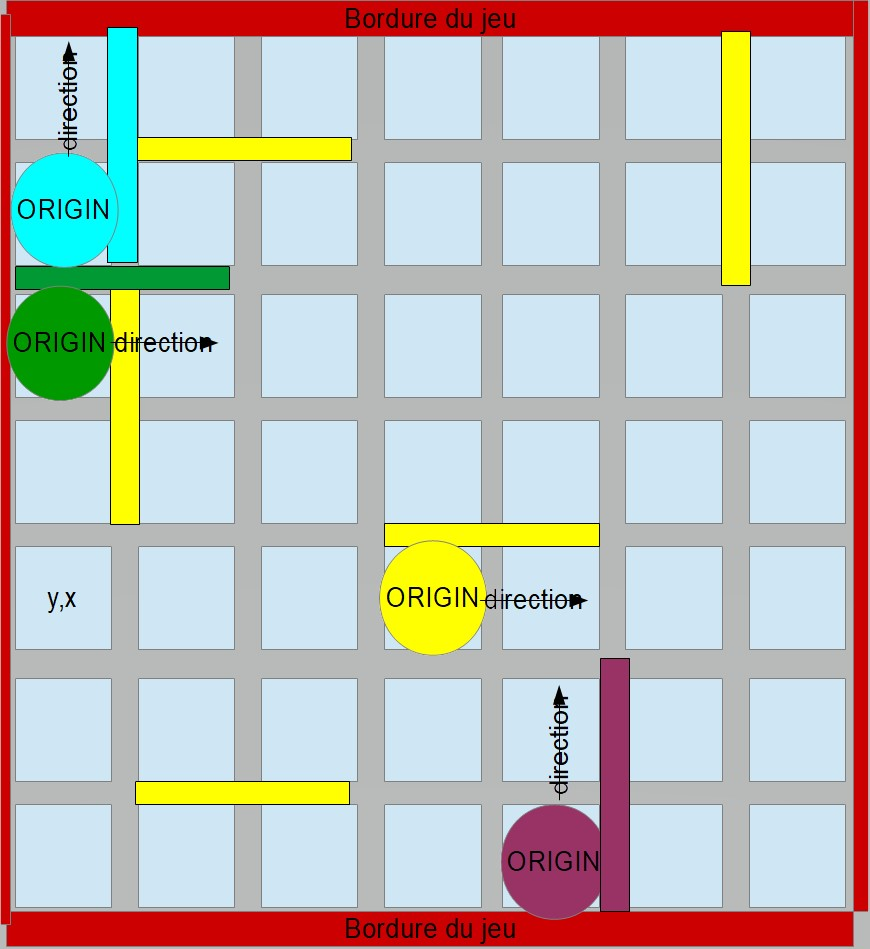
\includegraphics[scale=0.3]{wall.jpg} \\
\textit{Illustration du placement des murs.}
\end{center}
Avec cette convention, nous sommes sûr de pouvoir poser tout les murs possibles et imaginables. De plus, elle nous donne des hypothèses utiles pour l'implémentation des règles. Les murs étant stocké par le plateau dans une liste dont chaque élément est un tableau composé de la coordonnée d'origine du mur et de celle de la deuxième case à laquelle il est attaché, on peut grâce à ça facilement déterminer si c'est un mur vertical ou horizontal. On peut également aisément voir grâce à se format si deux cases adjacentes ont un mur continu sur leur côté ou non. Pour le savoir il suffit de regarder dans la liste des murs s'il existe un tableau composé de d'abord la coordonnée de la case avec le plus petit abscisse ou la plus grande ordonnée suivi en dernière position de la coordonnée de l'autre case.

\subsection{Structure du modèle}
Une chose qu'il a fallu clarifier tôt dans le développement est la structure du modèle.
Nous avons décider d'opter pour un objet \textit{Game} qui allait contenir touts les éléments de la partie en cours. Ce qu'il nous faut pour le jeu de base, c'est un plateau, des pions et des murs. Mais dans un but de modularité et pour pouvoir dans le futur rajouter des fonctionnalités, nous avons créer des catégories qui donneront nos packages :
\begin{itemize}
\item[•] \textit{world} : contient tout ce qui est relatif au monde dans lequel le jeu se déroule, dans notre cas c'est un simple plateau et des cases.
\item[•] \textit{item} : contient tout les éléments du jeu, toutes les pièces comme les pions et les murs mais pourquoi pas des outils ou des power-up dans le futur ?
\item[•] \textit{controller} : contient les entités chargées de contrôler les \textit{items}, par exemple, un PawnController est conçu pour pouvoir contrôler un pion et rien d'autre.
\item[•] \textit{engine} : contient tout ce qui est relatif à la logique de jeu ou le bon fonctionnement de celui-ci comme les règles mais aussi le jeu lui-même, les différentes IA et le système de sauvegarde.
\item[•] \textit{tool} : ce package un peu spécial contient des outils généraux qui servent à de multiples endroits dans le projet. Pour l'instant, il ne contient que la classe de coordonnées.
\item[•] \textit{gui} : c'est ce package qui va s'occuper de toute l'interface utilisateur mais aussi de la gestion du joueur humain.
\end{itemize}
Cela c'est avéré être une base solide. Nous avons avec ça mis au point une hiérarchie simple pour \textit{item} et \textit{controller} où ces deux packages contiennent chacun une classe abstraite mère qui représente l'élément le plus basique possible dans sa catégorie. Chaque autre classes héritent de leur classe mère afin de s'assurer que chacun ai le minimum syndicale pour être dans le jeu.

\subsection{Le pathfinding}
Tout les chemins mènent à Rome mais aussi tout les moyens de transports ! Il a donc fallu choisir entre les différentes façon de trouver le chemin le plus courts. \\
Dans sa thèse \textit{Mastering Quoridor}, Lisa GLENDENNING explique qu'elle a choisi de voir le plateau comme un graphe et utilise donc \href{https://en.wikipedia.org/wiki/Dijkstra_algorithm}{l'algorithme de Dijkstra}. Nous avons donc envisagée cette option mais bien qu'efficace elle nous semblait trop difficile à implémenter. Nous avons finalement opté pour l'algorithme présenté en séance par les assistants : le \href{https://en.wikipedia.org/wiki/Breadth-first_search}{breadth-first search} \textit{i.e} le parcours en largeur.

\subsection{La GUI}
Résolution 600x600 -> pourquoi ?

\section{Algorithme}

\subsection{Le pathfinding}
Comme dis précédemment, nous avons choisis d'implémenter le \textit{breadth-first search}. \\
L'idée est donc de partir du pion et d'explorer toute les cases possible aux alentours. Ensuite, toutes ses cases nouvellement explorées doivent être explorées à leur tour et ainsi de suite jusqu'à ce qu'on ai trouvé un case qui rempli la condition de victoire. Etant donnée que chaque case renvoie vers la case depuis laquelle on l'a explorée, on peut ensuite remonté jusqu'au pion et nous avons notre chemin le plus court. \\
Pour implémenter ceci il a fallu d'abord définir une liste de cases que l'on a déjà explorée et une liste contenant les cases qui doivent être explorées à la prochaine itération. \\
L'algorithme principale (findAPath) initialise les différentes listes ainsi qu'une HashTable qui va contenir les liens entre les cases. Dans cette table, la clé est une case et la valeur associé renvoie vers la case dont on est venu. La case de départ est marquée avec une coordonnée spéciale, de même pour la case d'arrivée. L'algorithme va ensuite lancer des itérations (explore) pour explorer les cases aux alentours en vérifiant qu'on explore pas deux fois la même case et qu'on respecte bien les règles de déplacement.

\subsection{Les règles}
Les règles n'ont pas toute été simples à implémenter. Autant la validité d'un déplacement ne demande que de vérifier si la case où l'on se trouve possède un mur dans la direction donnée autant tester la validité d'un mur est autrement plus complexe. \\
Je cite la règle officielle quant au placement des murs : \\
\textit{"La pose des barrières a pour but de se créer son propre chemin ou de ralentir l’adversaire, mais il est interdit de lui fermer totalement l’accès à sa ligne de but: il faut toujours lui laisser une solution."} \\
Cela implique de vérifier lorsqu'on souhaite placer un mur qu'il existe encore un chemin pour chaque joueur en jeux. Pour vérifier cette règle, nous copions le plateau (qui contient également les murs et les pions), nous plaçons le mur voulu et pour chaque pions nous appliquons le pathfinding. Si celui-ci ne trouve pas de chemin alors on ne peux pas placer le mur en question.\\
Ceci dit une autre vérification doit être faite : \\
On ne doit pas chevaucher et/ou couper un mur existant et/ou poser un mur en partie ou totalement hors du plateau.
Grâce à la convention prise, nous pouvons aisément empêcher les murs de sortir. En effet il suffit d'empêcher de poser des murs attachés aux cases d'ordonnée 0 et celles d'abscisse t-1. Pour éviter tout chevauchement voici la méthode utilisée.\\
\textbf{Premier cas :} \\
 Soit notre mur représenté par [(y, x1),(y, x2)]\footnote{rappel : x1 = x2-1} il y a chevauchement dans les cas où les murs suivant existent dans la liste des murs du plateau :
\begin{itemize}
\item[•] [(y, x1),(y, x2)]
\item[•] [(y, x1-1),(y, x1)]
\item[•] [(y, x2),(y, x2+1)]
\end{itemize}
\textbf{Deuxième cas :} \\
 Soit notre mur représenté par [(y1, x),(y2, x)]\footnote{rappel : y2 = y1-1} il y a chevauchement dans les cas où les murs suivant existent dans la liste des murs du plateau :
\begin{itemize}
\item[•] [(y1, x),(y2, x)]
\item[•] [(y1+1, x),(y1, x)]
\item[•] [(y2, x),(y2-1, x)]
\end{itemize}
Ceci fait il ne reste plus qu'à vérifier que l'on ne coupe pas un mur déjà existant : \\
Pour cela, nous devons simulé le mur qui pourrait poser problème. Pour ce faire nous prenons la direction complémentaire\footnote{Up si le mur que l'on souhaite placer va vers la droite, Right sinon}, un créer un mur dont l'origine est la même que le mur que l'on veut placer mais dont la seconde partie est donnée par l'origine + la direction supplémentaire. Il suffit ensuite de regarder si un tel mur est déjà dans la liste des murs du plateau. Si oui on ne peut placer le mur désiré. \\
Dans un soucis d'optimisation, on vérifie d'abord les collisions avec d'autres murs ou les bords du plateau avant de vérifier s'il reste encore un chemin étant donnée que la complexité du pathfinding est plus élevée que les vérifications de collision.

\subsection{Les IAs}
blablabla IA...
\section{Problèmes survenus}
blablabla les ia, javaFX 

\section{Conclusion}

voilà, Virgil et Simon out.

\section{Bibliographie}
\begin{itemize}
\item \emph{Lisa GLENDENNING}, \textit{Mastering Quoridor},Albuquerque Nouveau Mexique, mai 2005.
\item Documentation du JDK 13 par Oracle, \url{https://docs.oracle.com/en/java/javase/13/docs/api/index.html}, consultée tout au long du projet.
\item Documentation de JavaFX 8 par Oracle, \url{https://docs.oracle.com/javase/8/javafx/api/toc.htm}, consultée tout au long du projet.
\item Documentation de la JavaDoc par Oracle, \url{https://www.oracle.com/technical-resources/articles/java/javadoc-tool.html#tag}, consultée tout au long du projet.
\end{itemize}

\section{Remerciements}

Nous tenons à remercier en premier lieu les assistants du cours de Programmation et algorithmique 1 et 2 pour leurs réponses claires à nos question.
Également merci à Guillaume Proot pour tout ses précieux conseils et retour sur certaines parties de notre projet.
Monsieur Mélot, merci de nous avoir permis d'utiliser la classe \textit{CpuTime} afin d'encore et toujours améliorer notre projet.






























\end{document}
